\subsubsection*{RS232 to RS485} \label{sec:RS485}
The radio module and robot runs with two different communication standards. Therefore a conversion unit between the two standards is needed,this project uses the BOB-10124 to handle the conversion. 
\begin{figure}[H]
    \centering
    

\tikzset{every picture/.style={line width=0.75pt}} %set default line width to 0.75pt        

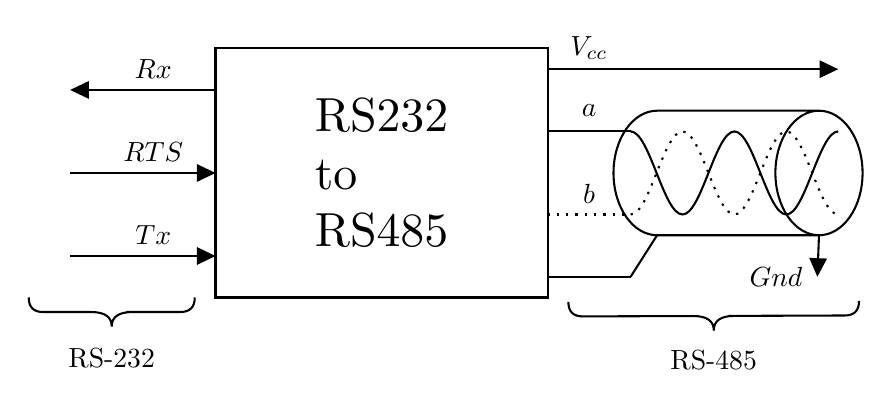
\begin{tikzpicture}[x=0.75pt,y=0.75pt,yscale=-1,xscale=1]
%uncomment if require: \path (0,217.6363525390625); %set diagram left start at 0, and has height of 217.6363525390625

%Shape: Rectangle [id:dp992532621229332] 
\draw   (100,30) -- (260,30) -- (260,150) -- (100,150) -- cycle ;
%Straight Lines [id:da5747180744657265] 
\draw    (32,50) -- (100,50) ;

\draw [shift={(30,50)}, rotate = 0] [fill={rgb, 255:red, 0; green, 0; blue, 0 }  ][line width=0.75]  [draw opacity=0] (8.93,-4.29) -- (0,0) -- (8.93,4.29) -- cycle    ;
%Straight Lines [id:da22964301218996663] 
\draw    (30,90) -- (98,90) ;
\draw [shift={(100,90)}, rotate = 180] [fill={rgb, 255:red, 0; green, 0; blue, 0 }  ][line width=0.75]  [draw opacity=0] (8.93,-4.29) -- (0,0) -- (8.93,4.29) -- cycle    ;

%Straight Lines [id:da2677261187564559] 
\draw    (30,130) -- (98,130) ;
\draw [shift={(100,130)}, rotate = 180] [fill={rgb, 255:red, 0; green, 0; blue, 0 }  ][line width=0.75]  [draw opacity=0] (8.93,-4.29) -- (0,0) -- (8.93,4.29) -- cycle    ;

%Straight Lines [id:da5541489716106782] 
\draw  [dash pattern={on 0.84pt off 2.51pt}]  (260,110) -- (300,110) ;


%Straight Lines [id:da09956683895016183] 
\draw    (260,70) -- (300,70) ;


%Shape: Wave [id:dp6378387303335409] 
\draw  [dash pattern={on 0.84pt off 2.51pt}] (300,110) .. controls (304.52,110) and (308.42,100.25) .. (312.5,90) .. controls (316.58,79.75) and (320.48,70) .. (325,70) .. controls (329.52,70) and (333.42,79.75) .. (337.5,90) .. controls (341.58,100.25) and (345.48,110) .. (350,110) .. controls (354.52,110) and (358.42,100.25) .. (362.5,90) .. controls (366.58,79.75) and (370.48,70) .. (375,70) .. controls (379.52,70) and (383.42,79.75) .. (387.5,90) .. controls (391.58,100.25) and (395.48,110) .. (400,110) ;
%Shape: Wave [id:dp12967964362630724] 
\draw   (300,70) .. controls (304.52,70) and (308.42,79.75) .. (312.5,90) .. controls (316.58,100.25) and (320.48,110) .. (325,110) .. controls (329.52,110) and (333.42,100.25) .. (337.5,90) .. controls (341.58,79.75) and (345.48,70) .. (350,70) .. controls (354.52,70) and (358.42,79.75) .. (362.5,90) .. controls (366.58,100.25) and (370.48,110) .. (375,110) .. controls (379.52,110) and (383.42,100.25) .. (387.5,90) .. controls (391.58,79.75) and (395.48,70) .. (400,70) ;
%Straight Lines [id:da2654543253939561] 
\draw    (260,140) -- (300,140) ;


%Flowchart: Direct Access Storage [id:dp6439756816416224] 
\draw   (390.75,120) -- (312.75,120) .. controls (301.15,120) and (291.75,106.57) .. (291.75,90) .. controls (291.75,73.43) and (301.15,60) .. (312.75,60) -- (390.75,60)(411.75,90) .. controls (411.75,106.57) and (402.35,120) .. (390.75,120) .. controls (379.15,120) and (369.75,106.57) .. (369.75,90) .. controls (369.75,73.43) and (379.15,60) .. (390.75,60) .. controls (402.35,60) and (411.75,73.43) .. (411.75,90) ;
%Straight Lines [id:da25800191363461744] 
\draw    (300,140) -- (312.75,120) ;


%Straight Lines [id:da7111201241992133] 
\draw    (390.75,120) -- (390.07,138) ;
\draw [shift={(390,140)}, rotate = 272.15] [fill={rgb, 255:red, 0; green, 0; blue, 0 }  ][line width=0.75]  [draw opacity=0] (8.93,-4.29) -- (0,0) -- (8.93,4.29) -- cycle    ;

%Straight Lines [id:da28410671201626836] 
\draw    (260,40) -- (398,40) ;
\draw [shift={(400,40)}, rotate = 180] [fill={rgb, 255:red, 0; green, 0; blue, 0 }  ][line width=0.75]  [draw opacity=0] (8.93,-4.29) -- (0,0) -- (8.93,4.29) -- cycle    ;

%Shape: Brace [id:dp2909486698907142] 
\draw   (10,150) .. controls (10,154.67) and (12.33,157) .. (17,157) -- (40,157) .. controls (46.67,157) and (50,159.33) .. (50,164) .. controls (50,159.33) and (53.33,157) .. (60,157)(57,157) -- (83,157) .. controls (87.67,157) and (90,154.67) .. (90,150) ;
%Shape: Brace [id:dp6537232873413532] 
\draw   (270,152.14) .. controls (270.01,156.81) and (272.35,159.13) .. (277.02,159.11) -- (330.05,158.93) .. controls (336.72,158.9) and (340.06,161.22) .. (340.07,165.89) .. controls (340.06,161.22) and (343.38,158.88) .. (350.05,158.86)(347.05,158.87) -- (403.07,158.67) .. controls (407.74,158.66) and (410.06,156.32) .. (410.05,151.65) ;

% Text Node
\draw (70,40) node   {$Rx$};
% Text Node
\draw (70,80) node   {$RTS$};
% Text Node
\draw (70,120) node   {$Tx$};
% Text Node
\draw (180,90) node [scale=1.7280000000000002] [align=left] {RS232\\to\\RS485};
% Text Node
\draw (280,60) node   {$a$};
% Text Node
\draw (280,100) node   {$b$};
% Text Node
\draw (370,140) node   {$Gnd$};
% Text Node
\draw (280,30) node   {$V_{cc}$};
% Text Node
\draw (49.95,179.36) node  [align=left] {RS-232};
% Text Node
\draw (340,180) node  [align=left] {RS-485};


\end{tikzpicture}

    \caption{RS232 to RS485 conversion}
    \label{fig:RSPROTO}
\end{figure}
\noindent
The two communication-systems are both standards for serial communication. However the RS-232 only supports point to point(PTP) transmitting and receiving, while RS-485 can handle the communication of up to 32 devices and the speed can be set significantly higher. A system utilising RS-232 can transmit at $20 Kbits/s$ where a system with RS-485 can transmit at $10 Mbits/s$. The length of the data transmission inside a cable is also higher with RS-485 where the system can run on a $1200 m$ cable, while RS-232 can only cover just under $16$ meters of cable. \\
The use of cable in this project do not exceed the cable length supported by RS-232. However, there is a need to daisy chain the 5 servo motors on the robot which is the main reason why there is a conversion between the RS-232 used by the XBee and RS-485 used by the Dynamixel servos.\\

%To communicate between the Teensy and the Dynamixel servos, there is a need for a conversion from the RS-232 protocol to the RS-485. This conversion is due to the fact that the Teensy uses the RS-232 protocol as communication and the servos utilises the Rs485 protocol.\\
\noindent
RS-232 can receive and transmit at the same time, making it full dupelx, however since it is chained to a system running with a 2-wired-RS-485 it only reads or transmits, which means it is half duplex. The signal the RS-232 send is 8-bit and purely zeroes and ones. The signal is idle on 1, so when the bit goes to zero the start is initiated. The 9600N1 is the checksum of the system and disregards uneven parity, which means that bit-streams with, e.g, 3 1's will not be read. \\
\noindent
The RS-485 is the differential signal between the two signals A and B, where the difference decides whether it is a 0 or a 1 being sent.\\
The RS-485 consists of two lines that often, but not in this case, is twisted together for higher noise immunity. The first line, A, is low for 0 and high for 1, while the other line, B, is the inverted signal, that is high for 1 and low for 0. As mentioned above, the system used in this project is using the two wired configuration of RS-485, where the system is half duplex.  \cite{RS232/485:online}


